\subsection{Internal waves}

% TODO: mention horizontal viscosities, energy? amplitude spectrum?

The breaking of nonlinear internal waves in the ocean is a significant source of abyssal mixing, and thus is an important process contributing to the abyssal ocean circulation \citep{nikurashin13}.

- but linear waves should involve no mixing

Spurious mixing due to internal waves depends strongly on the choice of vertical coordinate. The propagation of linear internal waves produces vertical mixing in ocean models with a fixed vertical grid such as z-star \citep{gouillon10}. However, other coordinates, such as z-tilde, permit layers to move with the waves, thereby restricting transport between layers and reducing spurious mixing.

\begin{figure}
  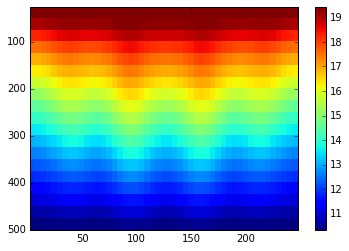
\includegraphics{{../plots/internal_waves_snapshot_0.01}.pdf}
  \caption{\label{fig:waves-snapshot} Snapshot of the internal wave initial condition (top), and state after 100 days (bottom). Temperature (\si{\celsius}) is shown in colours.}
\end{figure}

- show z-tilde and rho coords as well (4-panel)

This test case is configured as presented by \citet{ilicak12}. It consists of a linearly stratified background temperature distribution in a domain \SI{500}{\metre} deep and \SI{250}{\kilo\metre} wide (\cref{fig:waves-snapshot}). Horizontal grid spacing is \SI{5}{\kilo\metre}, and the vertical grid spacing $\Delta z$ is \SI{25}{\metre}. A wave perturbation is superimposed, lifting the isopycnals in the centre of the domain to set up counter-propagating internal waves towards the left and right horizontal boundaries. The background temperature distribution is defined as

\begin{equation}
  \Theta_0(z) = \Theta_\text{bot} + (\Theta_\text{top} - \Theta_\text{bot})\frac{z_\text{bot} - z}{z_\text{bot}},
\end{equation}

where $\Theta_\text{bot} = 10.1^\circ\mathrm{C}$, $\Theta_\text{top} = \SI{20.1}{\celsius}$, and $z_\text{bot} = \SI{-487.5}{\metre}$. The wave perturbation,

- mention coordinate convention on z (z coordinate relative to surface)
- explain discrepancy in $z_\text{bot}$ due to staggered grid

\begin{equation}
  \Theta'(x,z) = -A\cos\left(\frac{\pi}{2L}(x - x_0)\right) \sin\left(\pi\frac{z + \Delta z/2}{z_\text{bot} + \Delta z/2}\right),
\end{equation}

is added in the region $x_0 - L < x < x_0 + L$, where $L = \SI{50}{\kilo\metre}$, $x_0 = \SI{125}{\kilo\metre}$. Only the high-amplitude case, with perturbation amplitude $A = \SI{2}{\celsius}$ is used, as it is the only case also presented by \citet{petersen15}. The waves set up by this perturbation have a period of approximately one day, so the test case is run for 100 days to allow the waves to propagate many times across the full extent of the domain.

- mention buoyancy frequency, or remove "propagation time"

\begin{figure}
  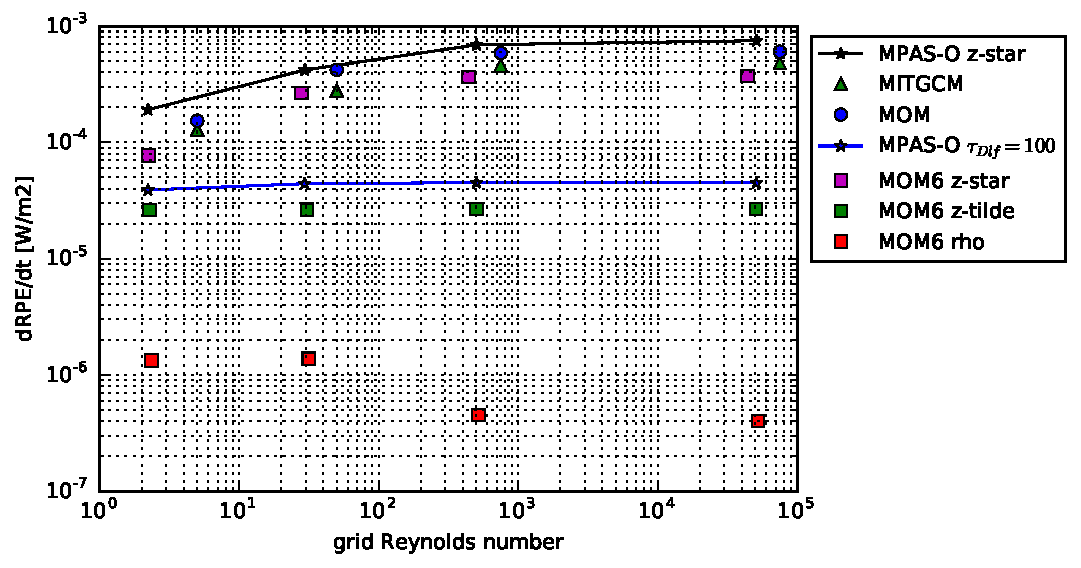
\includegraphics{../plots/internal_waves_drpe.pdf}
  \caption{\label{fig:waves-drpe} Averaged rate of RPE change from 10 to 100 days in internal waves test case. MPAS-O, MITGCM and MOM results come from \citet{petersen15} and \citet{ilicak12}. MOM6 is shown with square markers, in magenta for z-star, green for z-tilde and red for continuous isopycnal. MOM6 performs comparably or better to models using the same vertical coordinate, and shows a significant reduction in spurious mixing with the continuous isopycnal coordinate.}
\end{figure}

- state which results come from which model
- specify default MOM6 case is z-star

Considering the average rate of RPE change (\cref{fig:waves-drpe}), MOM6 performs well for each of the chosen vertical coordinates; z-star, z-tilde and continuous isopycnal (rho). This is likely due to its implementation as a quasi-Lagrangian ALE model. In this configuration, vertical layers are able to move freely within their column as waves pass through. During horizontal advection, there is exactly zero transport through vertical interfaces, so mixing occurs only laterally along an isopycnal layer. The vertical coordinate becomes more isopycnal with the z-tilde and rho coordinates, thus regridding causes smaller displacement of the interfaces. Subsequently, there is less vertical transport due to remapping and the overall spurious mixing is reduced.

The implementation of the z-tilde coordinate differs between MOM6 and MPAS-O. The filter timescale $\tau_{Dlf}$ in MPAS-O defines the cutoff above which frequencies are treated in a Lagrangian manner. As MOM6 is a layered model, all motion is Lagrangian during a single timestep. The only controllable parameter in the MOM6 implementation of z-tilde is $\tau_{hhf}$, which defines the relaxation timescale of the grid, to prevent long-term drift. We set this to 30 days to match the configuration used for MPAS-O. MOM6 exhibits only a modest improvement over MPAS-O here, since most dynamically interesting scales are already captured by the 100 day Lagrangian timescale $\tau_{Dlf}$ used by MPAS-O.

\subsubsection{Spurious mixing orientation}

\begin{figure}
  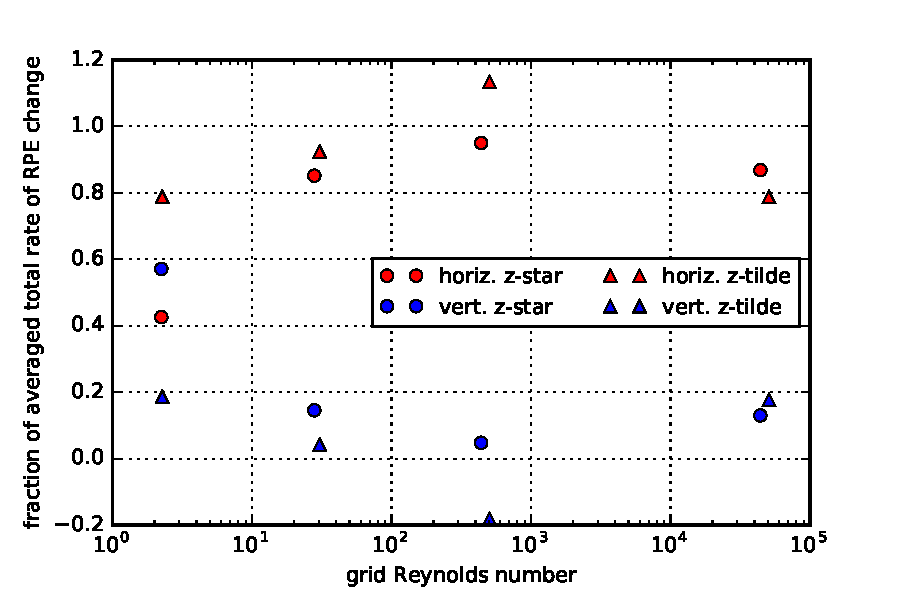
\includegraphics{../plots/internal_waves_drpe_split.pdf}
  \caption{\label{fig:waves-drpesplit} Relative contributions to spurious mixing by horizontal and vertical processes in internal waves test case. Each contribution is the fraction of the time-averaged total rate of RPE change.}
\end{figure}

- star symbol for z-star
- caption details

We take the z-star configuration of MOM6 (shown in magenta in \cref{fig:waves-drpe}) and compute the orientation of the spurious mixing, shown in \cref{fig:waves-drpesplit}. When $\mathrm{Re}_\Delta < 10$, the horizontal component is smaller than the vertical. This is consistent with the conclusion of \citet{ilicak12}, that the grid Reynolds number must be below 10 to avoid the saturation level of spurious mixing. In this regime, the vertical configuration such as coordinate or reconstruction accuracy can have a significant impact on the overall spurious mixing. There is a minimum in the vertical contribution at $\nu_h = \SI{1}{\square\metre\per\second}$, corresponding to $\mathrm{Re}_\Delta \approx 400$.

- why?

\Cref{fig:waves-drpesplit} shows the relative contributions to the total rate of RPE change by the horizontal and vertical components. There is once again a minimum in the contribution by the vertical component at $\nu_h = \SI{1}{\square\metre\per\second}$, corresponding to $\mathrm{Re}_\Delta \approx 400$. Since this also happens with the z-star and continuous isopycnal coordinates (\cref{fig:waves-drpe}), it is mostly likely a feedback effect or resonance due to the horizontal viscosity.
